% Source: Code/xband-radar-sim/docs/radar_simulation_technical.tex
% Description: Ray generation for a single azimuth. 2000 rays are distributed randomly within $\pm 1.5 \times$ beamwidth of boresight. Orange arrows show individual rays.

\documentclass[border=4pt]{standalone}
\usepackage{algpseudocode}
\usepackage{amsmath,amssymb,amsfonts}
\usepackage[T1]{fontenc}
\usepackage{graphicx}
\usepackage{pgfplots}
\usepackage{tikz}
\usepackage{xcolor}
\pgfplotsset{compat=1.18}
\usetikzlibrary{arrows.meta,positioning,shapes.geometric,calc,patterns,decorations.pathmorphing,3d,angles,quotes}

\definecolor{radargreen}{RGB}{0,255,0}
\definecolor{raycolor}{RGB}{255,165,0}
\definecolor{targetcolor}{RGB}{255,0,0}
\definecolor{groundcolor}{RGB}{139,90,43}
\definecolor{skycolor}{RGB}{135,206,235}
\definecolor{beamcolor}{RGB}{255,255,0}


\begin{document}
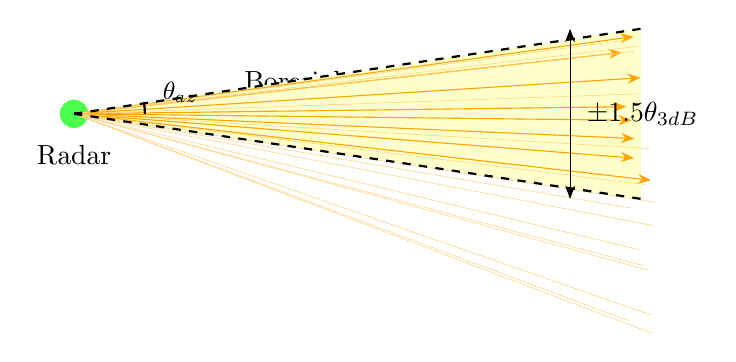
\begin{tikzpicture}[scale=0.9]
    % Radar
    \fill[green!70] (0,0) circle (0.2);
    \node[below] at (0,-0.3) {Radar};

    % Boresight direction
    \draw[-{Stealth}, very thick, black] (0,0) -- (8,0);
    \node[above] at (4,0.1) {Boresight ($\phi = 45°$)};

    % Beam cone (filled)
    \fill[beamcolor!20] (0,0) -- (8,1.2) -- (8,-1.2) -- cycle;

    % Individual rays
    \foreach \y in {-1.0,-0.7,-0.4,-0.1,0.2,0.5,0.8,1.1} {
        \pgfmathsetmacro{\randx}{0.3*rand}
        \draw[raycolor, thin, -{Stealth}] (0,0) -- ({8+\randx},{\y + 0.1*rand});
    }

    % More rays (denser)
    \foreach \i in {1,...,15} {
        \pgfmathsetmacro{\y}{-1.1 + 2.2*rand}
        \pgfmathsetmacro{\randx}{0.2*rand}
        \draw[raycolor!50, very thin] (0,0) -- ({8+\randx},{\y});
    }

    % Beam edges
    \draw[dashed, thick] (0,0) -- (8,1.2);
    \draw[dashed, thick] (0,0) -- (8,-1.2);

    % Beamwidth annotation
    \draw[{Stealth}-{Stealth}] (7,1.2) -- (7,-1.2);
    \node[right] at (7.1,0) {$\pm 1.5 \theta_{3dB}$};

    % Angle arc
    \draw[thick] (1,0) arc (0:8:1);
    \node at (1.5,0.3) {\small $\theta_{az}$};

\end{tikzpicture}
\end{document}
